\renewcommand{\theequation}{\theenumi}
\begin{enumerate}[label=\arabic*.,ref=\thesubsection.\theenumi]
\numberwithin{equation}{enumi}
\item Totalno of drivers taking part in survey = 2000
\\
no of drivers in the age 18-29 and having 3 accidents in a year = 61
\\
probability  of drivers in the age 18-29 and having 3 accidents in a year = P(X=1)\\
\begin{align}
P\left(X=1\right) &= \frac{61}{2000}
\\
&= 0.03
\end{align}
\\
\item no of drivers in the age 30-50 and having 1 or more accidents in a year = 125+60+22 = 207
\\
probability  of drivers in the age 30-50 and having 1 or more accidents in a year = P(X=2)\\
\begin{align}
P\left(X=2\right) &= \frac{207}{2000}
\\
&= 0.103
\end{align}
\item no of drivers having no accidents in a year = 440+505+360=1305
\\
probability  of drivers having no accidents in a year = P(X=3)\\
\begin{align}
P\left(X=3\right) &= \frac{1305}{2000}
\\
&= 0.65
\end{align}
codes for the above equation can be get from here
\begin{lstlisting}
codes/probexm/probexm8.py
\end{lstlisting}
\begin{figure}[!ht]
\centering
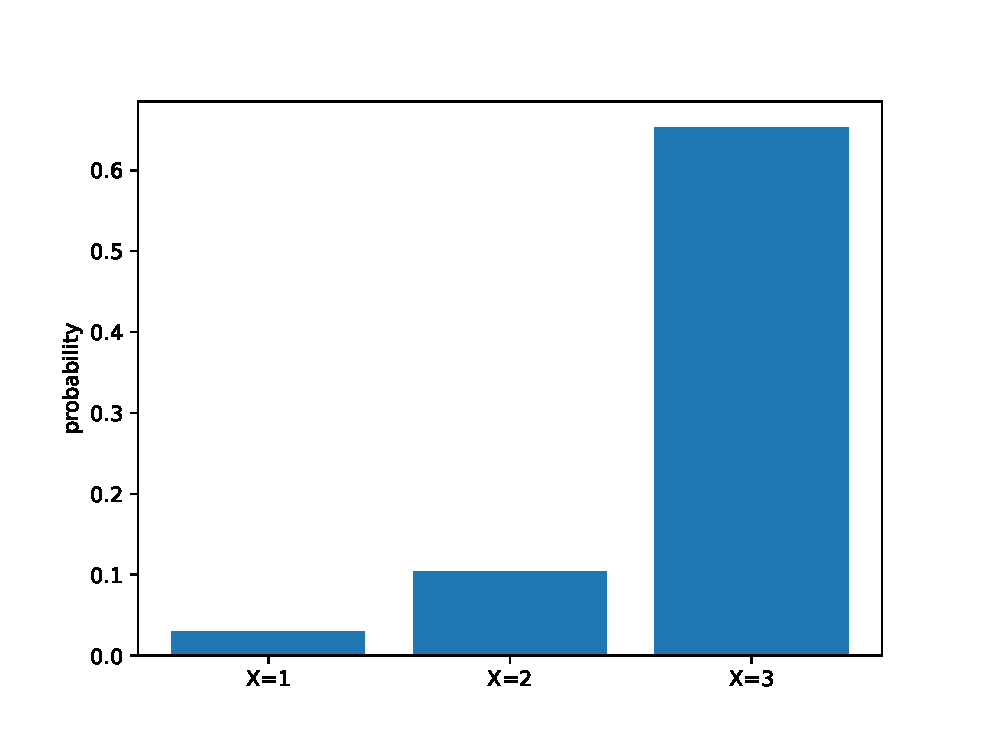
\includegraphics[width=\columnwidth]{./figures/probexm/probexm8.eps}
\caption{probability ofaccident in an year }
\label{fig:bt2}
\begin{lstlisting}
figs/probexm/probexm8.eps
\end{lstlisting}
\end{figure}
\end{enumerate}